% Options for packages loaded elsewhere
\PassOptionsToPackage{unicode}{hyperref}
\PassOptionsToPackage{hyphens}{url}
%
\documentclass[
]{article}
\title{Econometrie II : Transports}
\usepackage{etoolbox}
\makeatletter
\providecommand{\subtitle}[1]{% add subtitle to \maketitle
  \apptocmd{\@title}{\par {\large #1 \par}}{}{}
}
\makeatother
\subtitle{Rapport}
\author{Guewen HESLAN - Bijan VALILOU}
\date{Janvier 2021}

\usepackage{amsmath,amssymb}
\usepackage{lmodern}
\usepackage{iftex}
\ifPDFTeX
  \usepackage[T1]{fontenc}
  \usepackage[utf8]{inputenc}
  \usepackage{textcomp} % provide euro and other symbols
\else % if luatex or xetex
  \usepackage{unicode-math}
  \defaultfontfeatures{Scale=MatchLowercase}
  \defaultfontfeatures[\rmfamily]{Ligatures=TeX,Scale=1}
\fi
% Use upquote if available, for straight quotes in verbatim environments
\IfFileExists{upquote.sty}{\usepackage{upquote}}{}
\IfFileExists{microtype.sty}{% use microtype if available
  \usepackage[]{microtype}
  \UseMicrotypeSet[protrusion]{basicmath} % disable protrusion for tt fonts
}{}
\makeatletter
\@ifundefined{KOMAClassName}{% if non-KOMA class
  \IfFileExists{parskip.sty}{%
    \usepackage{parskip}
  }{% else
    \setlength{\parindent}{0pt}
    \setlength{\parskip}{6pt plus 2pt minus 1pt}}
}{% if KOMA class
  \KOMAoptions{parskip=half}}
\makeatother
\usepackage{xcolor}
\IfFileExists{xurl.sty}{\usepackage{xurl}}{} % add URL line breaks if available
\IfFileExists{bookmark.sty}{\usepackage{bookmark}}{\usepackage{hyperref}}
\hypersetup{
  pdftitle={Econometrie II : Transports},
  pdfauthor={Guewen HESLAN - Bijan VALILOU},
  hidelinks,
  pdfcreator={LaTeX via pandoc}}
\urlstyle{same} % disable monospaced font for URLs
\usepackage[margin=1in]{geometry}
\usepackage{longtable,booktabs,array}
\usepackage{calc} % for calculating minipage widths
% Correct order of tables after \paragraph or \subparagraph
\usepackage{etoolbox}
\makeatletter
\patchcmd\longtable{\par}{\if@noskipsec\mbox{}\fi\par}{}{}
\makeatother
% Allow footnotes in longtable head/foot
\IfFileExists{footnotehyper.sty}{\usepackage{footnotehyper}}{\usepackage{footnote}}
\makesavenoteenv{longtable}
\usepackage{graphicx}
\makeatletter
\def\maxwidth{\ifdim\Gin@nat@width>\linewidth\linewidth\else\Gin@nat@width\fi}
\def\maxheight{\ifdim\Gin@nat@height>\textheight\textheight\else\Gin@nat@height\fi}
\makeatother
% Scale images if necessary, so that they will not overflow the page
% margins by default, and it is still possible to overwrite the defaults
% using explicit options in \includegraphics[width, height, ...]{}
\setkeys{Gin}{width=\maxwidth,height=\maxheight,keepaspectratio}
% Set default figure placement to htbp
\makeatletter
\def\fps@figure{htbp}
\makeatother
\setlength{\emergencystretch}{3em} % prevent overfull lines
\providecommand{\tightlist}{%
  \setlength{\itemsep}{0pt}\setlength{\parskip}{0pt}}
\setcounter{secnumdepth}{5}
\usepackage{fancyhdr}
\pagestyle{fancy}
\fancyfoot[CO,CE]{Econométrie II}
\fancyfoot[LE,RO]{\thepage}
\usepackage{booktabs}
\usepackage{longtable}
\usepackage{array}
\usepackage{multirow}
\usepackage{wrapfig}
\usepackage{float}
\usepackage{colortbl}
\usepackage{pdflscape}
\usepackage{tabu}
\usepackage{threeparttable}
\usepackage{threeparttablex}
\usepackage[normalem]{ulem}
\usepackage{makecell}
\usepackage{xcolor}
\ifLuaTeX
  \usepackage{selnolig}  % disable illegal ligatures
\fi
\usepackage[]{biblatex}
\addbibresource{references.bib}

\begin{document}
\maketitle

\tableofcontents
\newpage

\hypertarget{introduction}{%
\section{Introduction}\label{introduction}}

L'objectif ce projet est d'expliquer la quantité de diesel consommée par
les camions à partir des autres variables proposées et d'effectuer des
prévisions à horizon 2025. Nous allons donc tenter de répondre à la
question suivante : quels déterminants agissent dans la formation de la
quantité de pétrole consommée par les camions ? Pour y répondre nous
allons proposé un modèle économétrique et le confronter à divers tests
afin d'évaluer sa validité.

\hypertarget{pruxe9sentation-des-donnuxe9es}{%
\section{Présentation des
données}\label{pruxe9sentation-des-donnuxe9es}}

Nous disposons d'un jeu de données comprenant huit séries réunissant des
données de 1985 à 2019.

\begin{table}[!h]

\caption{\label{tab:unnamed-chunk-4}Consommation de gazole des camions}
\centering
\fontsize{7}{9}\selectfont
\begin{tabu} to \linewidth {>{}r>{\raggedleft}X>{\raggedleft}X>{\raggedleft}X>{\raggedleft}X>{\raggedleft}X>{\raggedleft}X>{\raggedleft}X>{\raggedleft}X}
\toprule
\textbf{Année} & \textbf{Quantité transportée par routes} & \textbf{Quantité transportée par train} & \textbf{Prix du disel (euros/litre de diesel)} & \textbf{Quantité de diesel consommé (en milliers de tonnes)} & \textbf{PIB en monnaie constante (base 100=2014)} & \textbf{Indice des prix à la consommation (base 100=2015)} & \textbf{Quantité de diesel consommé des camions (en milliers de tonnes)} & \textbf{PIB en volume (en milliards d’euros 2014)}\\
\midrule
\textbf{1985} & 128.42 & 56.06 & 0.60 & 11467 & 7.576890e+11 & 61.28 & 7999.56 & 1253.77\\
\textbf{1986} & 134.60 & 52.69 & 0.52 & 12364 & 8.145960e+11 & 62.83 & 8378.00 & 1283.07\\
\textbf{1987} & 144.52 & 52.71 & 0.50 & 13309 & 8.559830e+11 & 64.90 & 8874.91 & 1315.94\\
\textbf{1988} & 161.11 & 52.95 & 0.49 & 14903 & 9.252150e+11 & 66.65 & 10083.36 & 1378.36\\
\textbf{1989} & 168.64 & 53.71 & 0.52 & 16472 & 9.971210e+11 & 68.98 & 11026.46 & 1438.23\\
\textbf{1990} & 197.02 & 52.24 & 0.54 & 17908 & 1.053546e+12 & 71.19 & 12847.49 & 1480.29\\
\textbf{1991} & 202.67 & 52.43 & 0.55 & 18729 & 1.091705e+12 & 73.48 & 13088.60 & 1495.80\\
\textbf{1992} & 208.34 & 51.18 & 0.53 & 19824 & 1.130983e+12 & 75.21 & 13520.35 & 1519.72\\
\textbf{1993} & 204.24 & 45.58 & 0.56 & 20711 & 1.142119e+12 & 76.80 & 13736.33 & 1510.17\\
\textbf{1994} & 219.27 & 48.87 & 0.59 & 21735 & 1.179867e+12 & 78.07 & 13944.66 & 1545.79\\
\textbf{1995} & 234.50 & 48.27 & 0.59 & 22869 & 1.218273e+12 & 79.47 & 14175.76 & 1578.35\\
\textbf{1996} & 238.55 & 50.11 & 0.65 & 23489 & 1.252266e+12 & 81.04 & 14106.16 & 1600.65\\
\textbf{1997} & 246.95 & 54.25 & 0.68 & 24566 & 1.292777e+12 & 82.02 & 14718.88 & 1638.05\\
\textbf{1998} & 257.65 & 54.10 & 0.64 & 25667 & 1.351896e+12 & 82.55 & 15658.43 & 1696.83\\
\textbf{1999} & 266.86 & 54.54 & 0.69 & 26667 & 1.400999e+12 & 83.00 & 16588.18 & 1754.89\\
\textbf{2000} & 276.86 & 57.73 & 0.85 & 27355 & 1.478585e+12 & 84.39 & 16920.64 & 1823.74\\
\textbf{2001} & 290.43 & 51.72 & 0.80 & 28684 & 1.538200e+12 & 85.77 & 16846.18 & 1859.92\\
\textbf{2002} & 293.38 & 51.29 & 0.77 & 29670 & 1.587829e+12 & 87.42 & 17155.59 & 1881.04\\
\textbf{2003} & 296.99 & 48.06 & 0.79 & 30081 & 1.630666e+12 & 89.25 & 17034.63 & 1896.53\\
\textbf{2004} & 314.90 & 46.35 & 0.88 & 30762 & 1.704019e+12 & 91.16 & 17539.55 & 1950.19\\
\textbf{2005} & 314.15 & 40.70 & 1.03 & 31048 & 1.765905e+12 & 92.76 & 17707.32 & 1982.63\\
\textbf{2006} & 327.61 & 41.18 & 1.07 & 31891 & 1.848151e+12 & 94.31 & 18073.35 & 2031.19\\
\textbf{2007} & 339.95 & 42.61 & 1.09 & 32958 & 1.941360e+12 & 95.71 & 17911.82 & 2080.44\\
\textbf{2008} & 327.44 & 40.44 & 1.27 & 32827 & 1.992380e+12 & 98.41 & 17474.79 & 2085.74\\
\textbf{2009} & 284.40 & 32.13 & 1.00 & 32881 & 1.936422e+12 & 98.49 & 16954.37 & 2025.81\\
\textbf{2010} & 300.40 & 29.96 & 1.15 & 33588 & 1.995289e+12 & 100.00 & 17245.84 & 2065.31\\
\textbf{2011} & 300.16 & 34.18 & 1.34 & 34049 & 2.058369e+12 & 102.11 & 17561.67 & 2110.59\\
\textbf{2012} & 283.45 & 32.55 & 1.40 & 34120 & 2.088804e+12 & 104.11 & 17591.77 & 2117.20\\
\textbf{2013} & 292.00 & 32.00 & 1.35 & 34272 & 2.117189e+12 & 105.01 & 17653.77 & 2129.40\\
\textbf{2014} & 288.50 & 32.20 & 1.28 & 34407 & 2.149765e+12 & 105.54 & 17703.04 & 2149.76\\
\textbf{2015} & 281.50 & 34.30 & 1.15 & 34803 & 2.198432e+12 & 105.58 & 17757.19 & 2173.69\\
\textbf{2016} & 287.70 & 32.60 & 1.11 & 34777 & 2.234129e+12 & 105.77 & 17809.40 & 2197.50\\
\textbf{2017} & 307.70 & 33.42 & 1.23 & 34690 & 2.297242e+12 & 106.86 & 18328.21 & 2247.86\\
\textbf{2018} & 317.30 & 31.98 & 1.44 & 33626 & 2.363306e+12 & 108.84 & 17270.02 & 2289.78\\
\textbf{2019} & 322.30 & 31.58 & 1.44 & 32770 & 2.437635e+12 & 110.05 & 16344.30 & 2331.98\\
\bottomrule
\end{tabu}
\end{table}

\begin{center}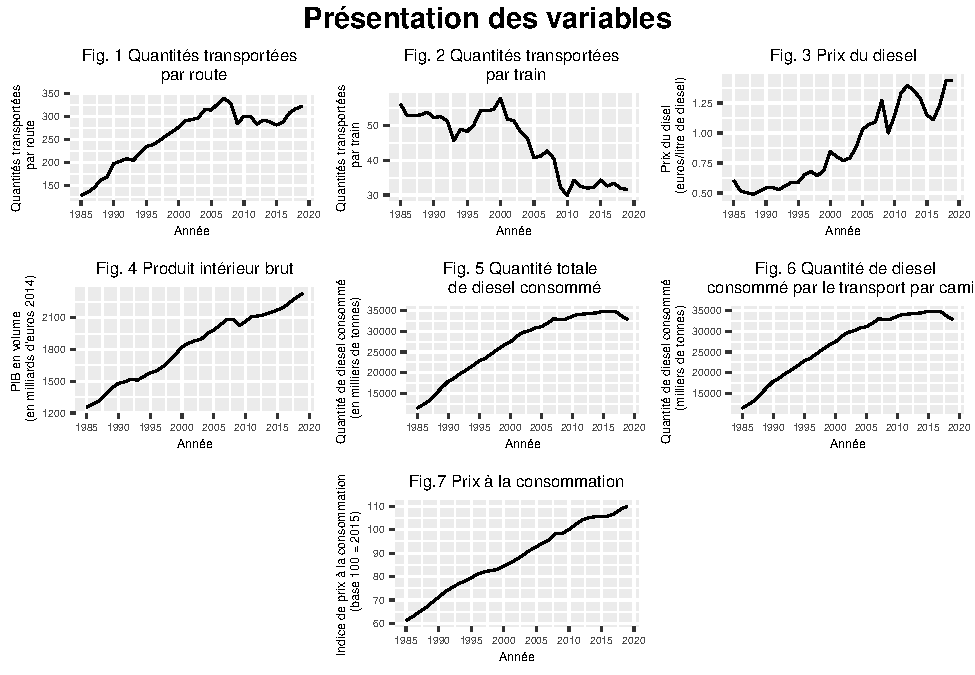
\includegraphics[width=1\linewidth,height=1\textheight]{Projet_econometrie_II_files/figure-latex/unnamed-chunk-5-1} \end{center}

\hypertarget{estimation-et-tests-du-premier-moduxe8le}{%
\section{Estimation et tests du premier
modèle}\label{estimation-et-tests-du-premier-moduxe8le}}

\hypertarget{les-variables-explicatives-choisies}{%
\subsection{Les variables explicatives
choisies}\label{les-variables-explicatives-choisies}}

Six variables sont proposées dans le but d'expliquer la quantité de
diesel consommée par les camions (sans compter l'ensemble des
transformations possibles). Afin d'obtenir un modèle pertinent nous
avons réalisé différents choix justifiés.

Nous avons immédiatement exclu la quantité de diesel consommée au total
qui comprend la variable que l'on tente d'expliquer : la consommation
globale de diesel semble davantage être une conséquence qu'une cause de
l'évolution de la quantité de diesel consommé par les camions.

On pourrait supposer que la quantité acheminée par rail soit le témoin
d'une substitution entre les différents modes d'acheminement des
marchandises. Même si le transport par route connaît une croissance
forte tandis que celui par rail décroît comme les figures 1 et 2 le
montrent, on peut observer la forte différence d'échelle entre les
utilisation des deux modes de transport. On remarque également que les
variations qui suivent après les années 2000 n'entraîne pas de réponse
significative sur l'une comme sur l'autre. L'évolution du transport
ferroviaire ne semble pas être un déterminant du transport routier, mais
une conséquence de l'évolution de facteurs structurels et politiques
comme Pierre Zembri l'a mis en lumière \autocite{zembri2004}.

Nous avons finalement choisis trois variables pour notre modèle :

\begin{enumerate}
    \item \textbf{La quantité de transport par route :} La consommation de diesel des camions est à la fois liés à la distance et à la masse de marchandises transportées.
    \item \textbf{Le PIB en volume :} L'indicateur principal de l'activité économique française.
    \item \textbf{Le prix du diesel déflaté:} On l'exprime également en volume : on pose le rapport entre prix nominal du diesel et indice des prix à la consommation pour obtenir le prix réel sur la base 2015.
\end{enumerate}

\hypertarget{uxe9quation-moduxe8le-et-ruxe9gression}{%
\subsection{Équation modèle et
régression}\label{uxe9quation-moduxe8le-et-ruxe9gression}}

\begin{equation}
    \label{eq:modele1}
    Q_{DCamion} = \beta_0 + \beta_1*\frac{P_{diesel}}{IPC} +  \beta_2*PIB + \beta_3*Q_{route} + \varepsilon
\end{equation}

Le premier modèle (1) suit l'équation avec les variables :

\begin{itemize}
\item
  \(Q_{DCamion}\) : La quantité de diesel consommée par les camions ;
\item
  \(PIB\) : Le PIB français en volume ;
\item
  \(P_{diesel}\) : Le prix du diesel ;
\item
  \(IPC\) : L'indice des prix à la consommation ;
\item
  \(Q_{route}\) : La quantité de marchandises transportées par route ;
\item
  \(\beta_n\) : Le coefficient associé à la n-ième variable explicative.
\end{itemize}

Toutes les variables obtenues sont significatives, car la probabilité
qu'elles soient nulles est inférieure à 5\%. La variable \(x1\) désigne
l'effet du prix du diesel, déflaté du niveau général des prix, qui a un
effet négatif très fort sur la consommation de diesel des camions. Le
gazole est donc un bien ordinaire, avec une élasticité-prix négative de
la demande. La variable \(x2\) représente l'effet du PIB mesuré en
volume. Le coefficient associé est positif, ce qui signifie que
l'augmentation du produit intérieur a un effet sectoriel positif sur le
secteur du transport par camion et donc de la consommation de gazole. La
variable \(x3\) vise la quantité de transport par route, qui a un effet
positif sur la consommation de diesel. Le coefficient de détermination
\(R^2\) est de \(94\%\), ce qui signifie une forte adéquation entre le
modèle et les données observées.

\begin{longtable}[]{@{}
  >{\centering\arraybackslash}p{(\columnwidth - 8\tabcolsep) * \real{0.25}}
  >{\centering\arraybackslash}p{(\columnwidth - 8\tabcolsep) * \real{0.15}}
  >{\centering\arraybackslash}p{(\columnwidth - 8\tabcolsep) * \real{0.18}}
  >{\centering\arraybackslash}p{(\columnwidth - 8\tabcolsep) * \real{0.14}}
  >{\centering\arraybackslash}p{(\columnwidth - 8\tabcolsep) * \real{0.17}}@{}}
\toprule
\begin{minipage}[b]{\linewidth}\centering
~
\end{minipage} & \begin{minipage}[b]{\linewidth}\centering
Estimate
\end{minipage} & \begin{minipage}[b]{\linewidth}\centering
Std. Error
\end{minipage} & \begin{minipage}[b]{\linewidth}\centering
t value
\end{minipage} & \begin{minipage}[b]{\linewidth}\centering
Pr(\textgreater\textbar t\textbar)
\end{minipage} \\
\midrule
\endhead
\textbf{(Intercept)} & 1767 & 790.8 & 2.235 & 0.03277 \\
\textbf{x1} & -378013 & 120267 & -3.143 & 0.003667 \\
\textbf{x2} & 4.242 & 1.423 & 2.98 & 0.005559 \\
\textbf{x3} & 36.89 & 5.615 & 6.57 & 2.449e-07 \\
\bottomrule
\end{longtable}

\begin{longtable}[]{@{}
  >{\centering\arraybackslash}p{(\columnwidth - 6\tabcolsep) * \real{0.21}}
  >{\centering\arraybackslash}p{(\columnwidth - 6\tabcolsep) * \real{0.31}}
  >{\centering\arraybackslash}p{(\columnwidth - 6\tabcolsep) * \real{0.12}}
  >{\centering\arraybackslash}p{(\columnwidth - 6\tabcolsep) * \real{0.24}}@{}}
\caption{Fitting linear model: y \textasciitilde{} x}\tabularnewline
\toprule
\begin{minipage}[b]{\linewidth}\centering
Observations
\end{minipage} & \begin{minipage}[b]{\linewidth}\centering
Residual Std. Error
\end{minipage} & \begin{minipage}[b]{\linewidth}\centering
\(R^2\)
\end{minipage} & \begin{minipage}[b]{\linewidth}\centering
Adjusted \(R^2\)
\end{minipage} \\
\midrule
\endfirsthead
\toprule
\begin{minipage}[b]{\linewidth}\centering
Observations
\end{minipage} & \begin{minipage}[b]{\linewidth}\centering
Residual Std. Error
\end{minipage} & \begin{minipage}[b]{\linewidth}\centering
\(R^2\)
\end{minipage} & \begin{minipage}[b]{\linewidth}\centering
Adjusted \(R^2\)
\end{minipage} \\
\midrule
\endhead
35 & 721.2 & 0.9475 & 0.9424 \\
\bottomrule
\end{longtable}

Nous allons effectuer un ensemble de tests sur le premier modèle estimer
afin de voir quelles manipulations sont nécessaires pour accroître la
validité du modèle.

\hypertarget{tests-de-stabilituxe9-temporelle}{%
\subsection{Tests de stabilité
temporelle}\label{tests-de-stabilituxe9-temporelle}}

Afin de détecter l'instabilité des coefficients dans un modèle de
régresson sans connaître la date a posteriori, nous allons effectuer un
test de Cusum proposé par Brown, Durbins et Evans (1975). Ce test repose
sur la somme cumulée réduites des résidus récursifs \(W_r\), ie
normalisée avec l'écart-type résiduel \(S_r\) :

\begin{equation}    
\label{eq:wr}    
W_r = \frac{1}{S} \overset{r}{\underset{i=K+1}{\sum}} w_j
\end{equation}

avec

\begin{equation}
\label{eq:S}

S = \sqrt{\frac{\overset{n}{\underset{i=1}{\sum}} \hat{\varepsilon}_i^2}{n - K}}
\end{equation}

En observant la figure 8, nous remarquons que \(W_r\) ne s'écarte pas
significativement de la droite \(W_r = 0\) et reste entre les deux
droites représentant le risque de première espèce \(\alpha\). Le
problème de ce test de ne pas prendre en compte le risque de deuxième
espèce.

\begin{center}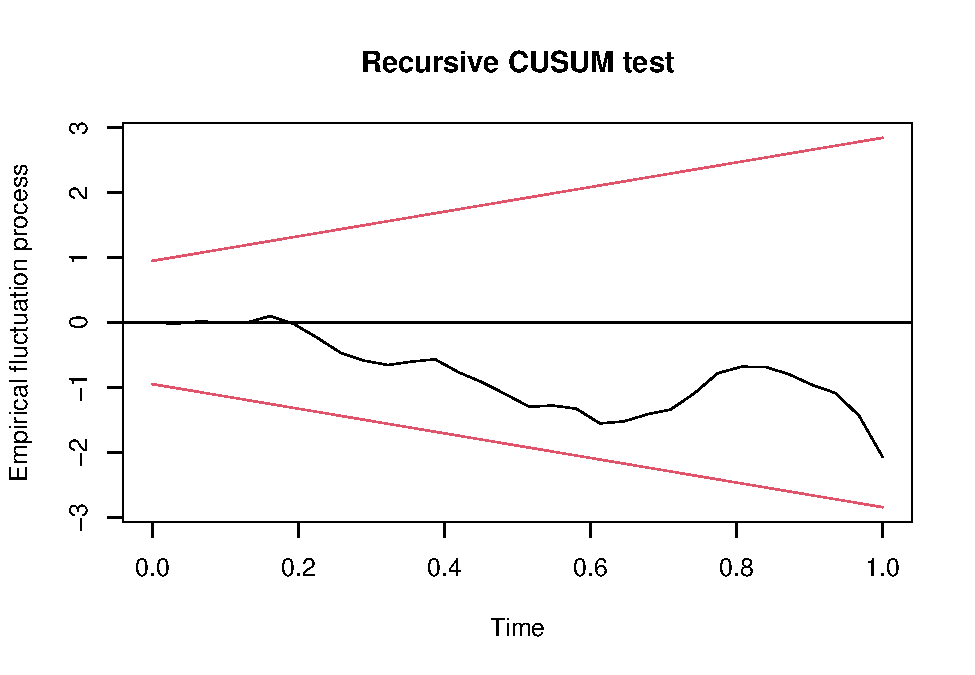
\includegraphics[width=0.7\linewidth,height=0.7\textheight]{Projet_econometrie_II_files/figure-latex/unnamed-chunk-7-1} \end{center}

Fig. 8 : Test de Cusum de stabilité temporelle du modèle 1

Le second test de Brown, Durbin et Evans (1975) est fondé sur le
Cusumsquare, ie les sommes des carrés résidus :

\begin{equation}
\label{eq:sr}
s_r = \frac{\overset{r}{\underset{i=K+1}{\sum}} w_j^2}{\overset{n}{\underset{i=K+1}{\sum}} w_j^2}
\end{equation}

Nous comparons la significativité de l'écart de \(s_r\) à son espérance
sous l'hypothèse nulle de constance des coefficients \(H_0\), grâce à un
couple de droites parallèles. Nous remarquons qu'à partir de 1998, la
statistique \(s_r\) est au-delà des valeurs limites.

\begin{center}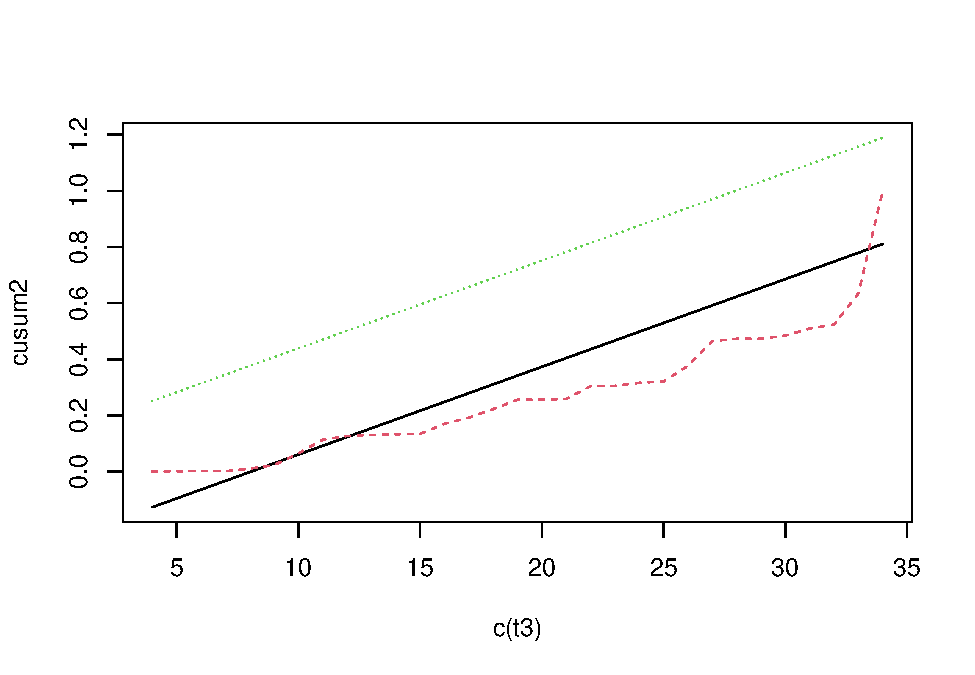
\includegraphics[width=0.7\linewidth,height=0.7\textheight]{Projet_econometrie_II_files/figure-latex/unnamed-chunk-8-1} \end{center}

Fig. 9 : Test de Cusumsquare de stabilité temporelle du modèle 1

Une fois que la période de rupture est approximativement estimée, nous
pouvons mettre en oeuvre le test de Chow (1960), qui permet de savoir si
les paramètres du modèle ont été modifiés à partir d'un rang
d'observation. Le test de Chow effectue une régression sur un
échantillon de \(n\) obervations (hypothèse nulle \(H_0\)) contre une
alternative de l'estimation du modèle sur deux sous-périodes \(n_1\) et
\(n_2\) avec \(n_1 + n_2 = n\). L'hypothèse nulle s'exprime sous la
forme :

\begin{equation}
\label{eq:H0chow}
H_0 : y = X\beta + \varepsilon 
\end{equation}

Le test de Chow calcul une statistique de Fischer fondée sur la somme
des carrés des résidisu sur l'échantillon complet \(SCR_0\) et la somme
des carrés des résidus du moèle alternatif \(SCR_1\) sur chaque
sous-période:

\begin{equation}
\label{eq:statF}
F(K,n-2K) = \frac{\frac{SCR_0 - SCR_1}{K}}{\frac{SCR_1}{n - 2K}}
\end{equation}

La p-value est-en dessous de 5\%, donc nous pouvons rejeter \(H_0\) de
la régression du modèle. Pour dater précisément l'année de rupture, il
faut évaluer la statistique de Fischer. Celle-ci est la plus élevée pour
l'année 2001, avec F= 11,39. La rupture a donc lieu en 2001.

\begin{table}[!h]

\caption{\label{tab:unnamed-chunk-9}Test de Chow de 1995 à 2004}
\centering
\fontsize{7}{9}\selectfont
\begin{tabu} to \linewidth {>{}l>{\raggedright}X>{\raggedright}X>{\raggedright}X>{\raggedright}X}
\toprule
\textbf{} & \textbf{statistic} & \textbf{p.value} & \textbf{method} & \textbf{data.name}\\
\midrule
\textbf{1995} & c(F = 4.64283563594701) & c(F = 0.00554738443120117) & Chow test & y \textasciitilde{} x\\
\textbf{1996} & c(F = 4.65133772559658) & c(F = 0.00549683616410357) & Chow test & y \textasciitilde{} x\\
\textbf{1997} & c(F = 5.79601334234664) & c(F = 0.0016800265235527) & Chow test & y \textasciitilde{} x\\
\textbf{1998} & c(F = 8.51147927330835) & c(F = 0.000140588189987745) & Chow test & y \textasciitilde{} x\\
\textbf{1999} & c(F = 10.7641179888783) & c(F = 2.38893676115515e-05) & Chow test & y \textasciitilde{} x\\
\textbf{2000} & c(F = 11.17276760355) & c(F = 1.77208419261943e-05) & Chow test & y \textasciitilde{} x\\
\textbf{2001} & c(F = 11.3979272051564) & c(F = 1.50725877964275e-05) & Chow test & y \textasciitilde{} x\\
\textbf{2002} & c(F = 10.5854028432303) & c(F = 2.72788003993218e-05) & Chow test & y \textasciitilde{} x\\
\textbf{2003} & c(F = 10.0026924784759) & c(F = 4.24242733156888e-05) & Chow test & y \textasciitilde{} x\\
\textbf{2004} & c(F = 9.93197977353754) & c(F = 4.48030603892313e-05) & Chow test & y \textasciitilde{} x\\
\bottomrule
\end{tabu}
\end{table}

\hypertarget{estimation-et-tests-de-stabilituxe9-temporelle-du-moduxe8le-2}{%
\section{Estimation et tests de stabilité temporelle du modèle
2}\label{estimation-et-tests-de-stabilituxe9-temporelle-du-moduxe8le-2}}

\hypertarget{estimation-du-moduxe8le-2-en-suxe9parant-les-variables-explicatives-par-sous-puxe9riode}{%
\subsection{Estimation du modèle 2 en séparant les variables
explicatives par
sous-période}\label{estimation-du-moduxe8le-2-en-suxe9parant-les-variables-explicatives-par-sous-puxe9riode}}

En observant la figure 3 (cf.~supra), le prix du diesel est la série
marquée par la plus grande variance. Nous essayons donc de séparer la
variable explicative prix du diesel sur deux sous-périodes : une allant
de 1985 à 2000 et l'autre de 2001 à 2019. Nous créons une nouvelle
variable \(\frac{P_{diesel}^{2001-2019}}{IPC^{2001-2019}}\) (toutes les
valeurs de la variable de 1985 à 2000 sont nulles) dissociée de la
variable \(\frac{P_{diesel}^{1985-2000}}{IPC^{1985-2000}}\) (toutes les
valeurs de la variable de 2001 à 2019 sont nulles).

\begin{equation}
    \label{eq:modele2}
    Q_{DCamion} = \beta_0 + \beta_1*\frac{P_{diesel}^{1985-2000}}{IPC^{1985-2019}} + \beta_2*\frac{P_{diesel}^{2001-2019}}{IPC^{2001-2019}} + \beta_3*PIB + \beta_4*Q_{route} + \varepsilon
\end{equation}

Toutes les variables obtenues sont significatives au seuil de 5\%. La
variable \(x1\) désigne l'effet du prix du diesel de 1985 à 2000 et la
variable \(x2\) l'effet du prix du diesel de 2001 à 2019. Le coefficient
associé est positif, ce qui signifie que l'augmentation du produit
intérieur a un effet sectoriel positif sur le secteur du transport par
camion et donc de la consommation de gazole. La variable \(x3\)
représnete le PIB en volume. La variable \(x4\) vise la quantité de
transport par route. Le coefficient de détermination \(R^2\) est de
\(94\%\), ce qui signifie une forte adéquation entre le modèle et les
données observées.

\begin{longtable}[]{@{}
  >{\centering\arraybackslash}p{(\columnwidth - 8\tabcolsep) * \real{0.25}}
  >{\centering\arraybackslash}p{(\columnwidth - 8\tabcolsep) * \real{0.15}}
  >{\centering\arraybackslash}p{(\columnwidth - 8\tabcolsep) * \real{0.18}}
  >{\centering\arraybackslash}p{(\columnwidth - 8\tabcolsep) * \real{0.14}}
  >{\centering\arraybackslash}p{(\columnwidth - 8\tabcolsep) * \real{0.17}}@{}}
\toprule
\begin{minipage}[b]{\linewidth}\centering
~
\end{minipage} & \begin{minipage}[b]{\linewidth}\centering
Estimate
\end{minipage} & \begin{minipage}[b]{\linewidth}\centering
Std. Error
\end{minipage} & \begin{minipage}[b]{\linewidth}\centering
t value
\end{minipage} & \begin{minipage}[b]{\linewidth}\centering
Pr(\textgreater\textbar t\textbar)
\end{minipage} \\
\midrule
\endhead
\textbf{(Intercept)} & 117.4 & 1670 & 0.07026 & 0.9445 \\
\textbf{x1} & -294623 & 141025 & -2.089 & 0.04528 \\
\textbf{x2} & -365083 & 120331 & -3.034 & 0.004947 \\
\textbf{x3} & 4.871 & 1.525 & 3.195 & 0.003283 \\
\textbf{x4} & 37.35 & 5.607 & 6.661 & 2.231e-07 \\
\bottomrule
\end{longtable}

\begin{longtable}[]{@{}
  >{\centering\arraybackslash}p{(\columnwidth - 6\tabcolsep) * \real{0.21}}
  >{\centering\arraybackslash}p{(\columnwidth - 6\tabcolsep) * \real{0.31}}
  >{\centering\arraybackslash}p{(\columnwidth - 6\tabcolsep) * \real{0.12}}
  >{\centering\arraybackslash}p{(\columnwidth - 6\tabcolsep) * \real{0.24}}@{}}
\caption{Fitting linear model: y \textasciitilde{} x}\tabularnewline
\toprule
\begin{minipage}[b]{\linewidth}\centering
Observations
\end{minipage} & \begin{minipage}[b]{\linewidth}\centering
Residual Std. Error
\end{minipage} & \begin{minipage}[b]{\linewidth}\centering
\(R^2\)
\end{minipage} & \begin{minipage}[b]{\linewidth}\centering
Adjusted \(R^2\)
\end{minipage} \\
\midrule
\endfirsthead
\toprule
\begin{minipage}[b]{\linewidth}\centering
Observations
\end{minipage} & \begin{minipage}[b]{\linewidth}\centering
Residual Std. Error
\end{minipage} & \begin{minipage}[b]{\linewidth}\centering
\(R^2\)
\end{minipage} & \begin{minipage}[b]{\linewidth}\centering
Adjusted \(R^2\)
\end{minipage} \\
\midrule
\endhead
35 & 718.3 & 0.9496 & 0.9429 \\
\bottomrule
\end{longtable}

\hypertarget{tests-de-stabilituxe9-temporelle-1}{%
\subsection{Tests de stabilité
temporelle}\label{tests-de-stabilituxe9-temporelle-1}}

Si on effectue un test de Cusumsquare , nous observons toujours une
instabilité temporelle comme le démontre la figure 10.

\begin{center}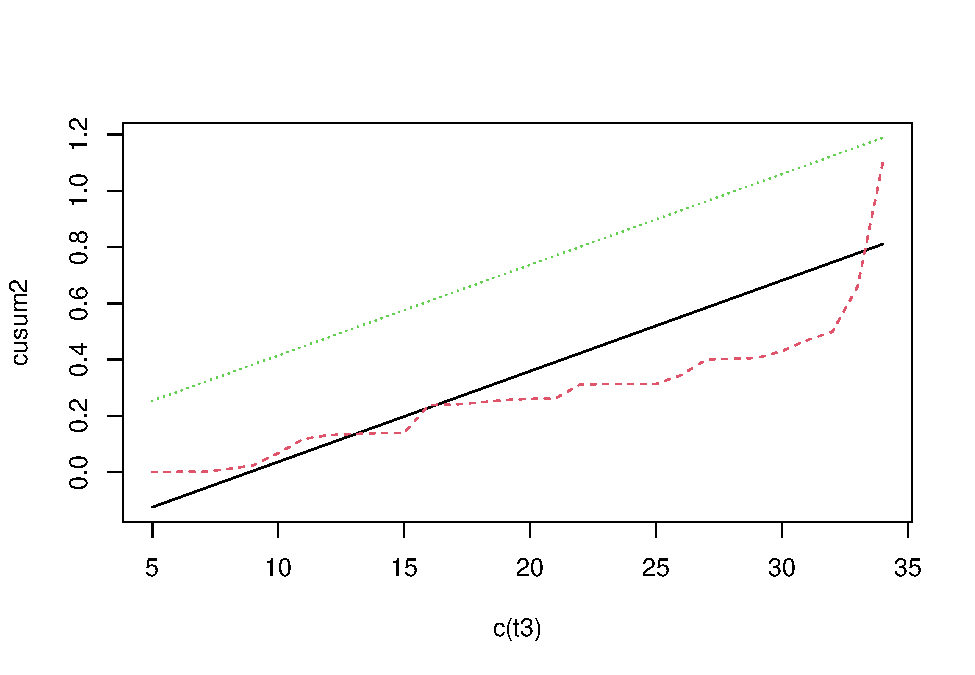
\includegraphics[width=0.7\linewidth,height=0.7\textheight]{Projet_econometrie_II_files/figure-latex/unnamed-chunk-11-1} \end{center}

Fig. 10 : Test de Cusumsquare de stabilité temporelle du modèle 2

Etant donné que le test de Chow ne fonctionne pas sur la fin de la série
temporelle en l'espèce, nous observons le comportement des résidus du
modèle (cf.~figure 11). Nous remarquons que les résidus du modèle en
valeur absolue augmentent durant les dernières années. La valeur réelle
de \(y\) est beaucoup plus forte que la valeur estimée par le modèle.
Nous pouvons donc supposer que le modèle a surestimé l'élasticité-prix
de la demande de gazole, car la période de 2017 à 2019 est associée à
une forte hausse des prix du carburant. La consommation n'a pas chuté,
car il s'agirait de dépenses contraintes pour les entreprises du secteur
des transport. Nous couperons donc la dernière valeur aberrante de
l'année 2019.

\begin{center}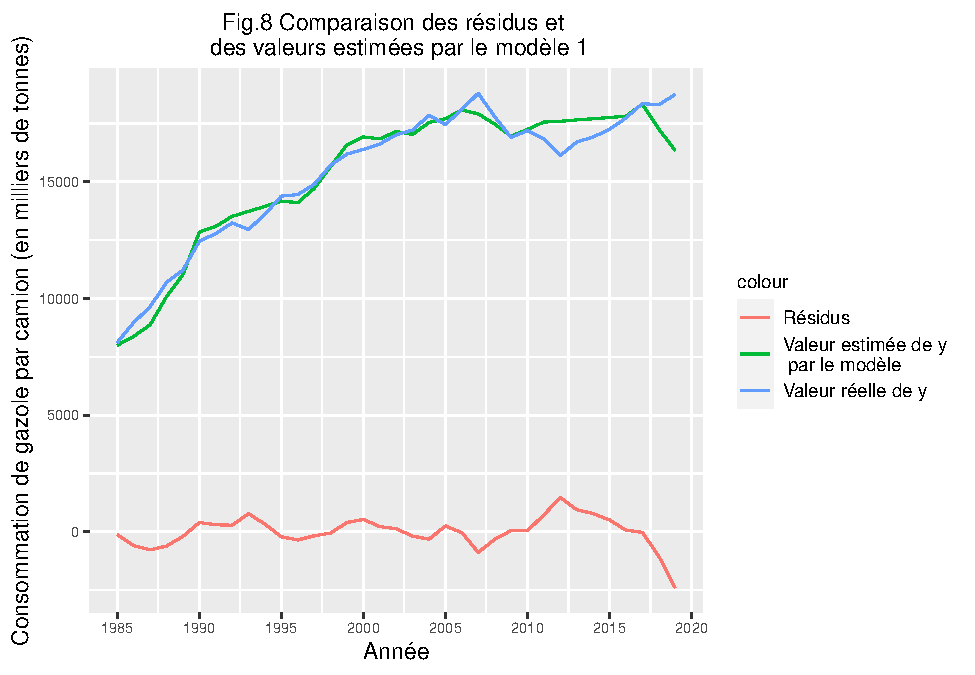
\includegraphics[width=0.7\linewidth,height=0.7\textheight]{Projet_econometrie_II_files/figure-latex/unnamed-chunk-12-1} \end{center}

Fig. 11 : Courbe des résidus

\hypertarget{estimation-et-tests-de-validituxe9-du-moduxe8le-3}{%
\section{Estimation et tests de validité du modèle
3}\label{estimation-et-tests-de-validituxe9-du-moduxe8le-3}}

\hypertarget{estimation-du-moduxe8le-3}{%
\subsection{Estimation du modèle 3}\label{estimation-du-moduxe8le-3}}

Il s'agit du même modèle présenté précédemment, mais sans la valeur de
l'année 2019.

\begin{equation}
    \label{eq:modele3}
    Q_{DCamion} = \beta_0 + \beta_1*\frac{P_{diesel}^{1985-2000}{IPC^{1985-2019}} + \beta_2*\frac{P_{diesel}^{2001-2018}{IPC^{2001-2018}} + \beta_3*PIB + \beta_4*Q_{route} + \varepsilon
\end{equation}

Les variables obtenues sont significatives au seuil de 5\%. La variable
\(x1\) désigne l'effet du prix du diesel de 1985 à 2000 et la variable
\(x2\) l'effet du prix du diesel de 2001 à 2019. Le coefficient associé
est positif, ce qui signifie que l'augmentation du produit intérieur a
un effet sectoriel positif sur le secteur du transport par camion et
donc de la consommation de gazole. La variable \(x3\) représnete le PIB
en volume. La variable \(x4\) vise la quantité de transport par route.
Le coefficient de détermination \(R^2\) de \(97\%\) est plus élevé que
pour les modèles 1 et modèle 2 .

\begin{longtable}[]{@{}
  >{\centering\arraybackslash}p{(\columnwidth - 8\tabcolsep) * \real{0.25}}
  >{\centering\arraybackslash}p{(\columnwidth - 8\tabcolsep) * \real{0.15}}
  >{\centering\arraybackslash}p{(\columnwidth - 8\tabcolsep) * \real{0.18}}
  >{\centering\arraybackslash}p{(\columnwidth - 8\tabcolsep) * \real{0.14}}
  >{\centering\arraybackslash}p{(\columnwidth - 8\tabcolsep) * \real{0.17}}@{}}
\toprule
\begin{minipage}[b]{\linewidth}\centering
~
\end{minipage} & \begin{minipage}[b]{\linewidth}\centering
Estimate
\end{minipage} & \begin{minipage}[b]{\linewidth}\centering
Std. Error
\end{minipage} & \begin{minipage}[b]{\linewidth}\centering
t value
\end{minipage} & \begin{minipage}[b]{\linewidth}\centering
Pr(\textgreater\textbar t\textbar)
\end{minipage} \\
\midrule
\endhead
\textbf{(Intercept)} & -1710 & 1328 & -1.288 & 0.208 \\
\textbf{x1} & -243723 & 107888 & -2.259 & 0.03157 \\
\textbf{x2} & -355441 & 91627 & -3.879 & 0.0005548 \\
\textbf{x3} & 6.237 & 1.196 & 5.217 & 1.389e-05 \\
\textbf{x4} & 34.15 & 4.321 & 7.902 & 1.026e-08 \\
\bottomrule
\end{longtable}

\begin{longtable}[]{@{}
  >{\centering\arraybackslash}p{(\columnwidth - 6\tabcolsep) * \real{0.21}}
  >{\centering\arraybackslash}p{(\columnwidth - 6\tabcolsep) * \real{0.31}}
  >{\centering\arraybackslash}p{(\columnwidth - 6\tabcolsep) * \real{0.12}}
  >{\centering\arraybackslash}p{(\columnwidth - 6\tabcolsep) * \real{0.24}}@{}}
\caption{Fitting linear model: y \textasciitilde{} x}\tabularnewline
\toprule
\begin{minipage}[b]{\linewidth}\centering
Observations
\end{minipage} & \begin{minipage}[b]{\linewidth}\centering
Residual Std. Error
\end{minipage} & \begin{minipage}[b]{\linewidth}\centering
\(R^2\)
\end{minipage} & \begin{minipage}[b]{\linewidth}\centering
Adjusted \(R^2\)
\end{minipage} \\
\midrule
\endfirsthead
\toprule
\begin{minipage}[b]{\linewidth}\centering
Observations
\end{minipage} & \begin{minipage}[b]{\linewidth}\centering
Residual Std. Error
\end{minipage} & \begin{minipage}[b]{\linewidth}\centering
\(R^2\)
\end{minipage} & \begin{minipage}[b]{\linewidth}\centering
Adjusted \(R^2\)
\end{minipage} \\
\midrule
\endhead
34 & 546.8 & 0.9717 & 0.9678 \\
\bottomrule
\end{longtable}

\hypertarget{tests-de-validituxe9}{%
\subsection{Tests de validité}\label{tests-de-validituxe9}}

\hypertarget{test-de-stabilituxe9-temporelle}{%
\subsubsection{Test de stabilité
temporelle}\label{test-de-stabilituxe9-temporelle}}

Le test de Cusumsquare décrit supra confirme l'absence de rupture dans
le modèle 3.

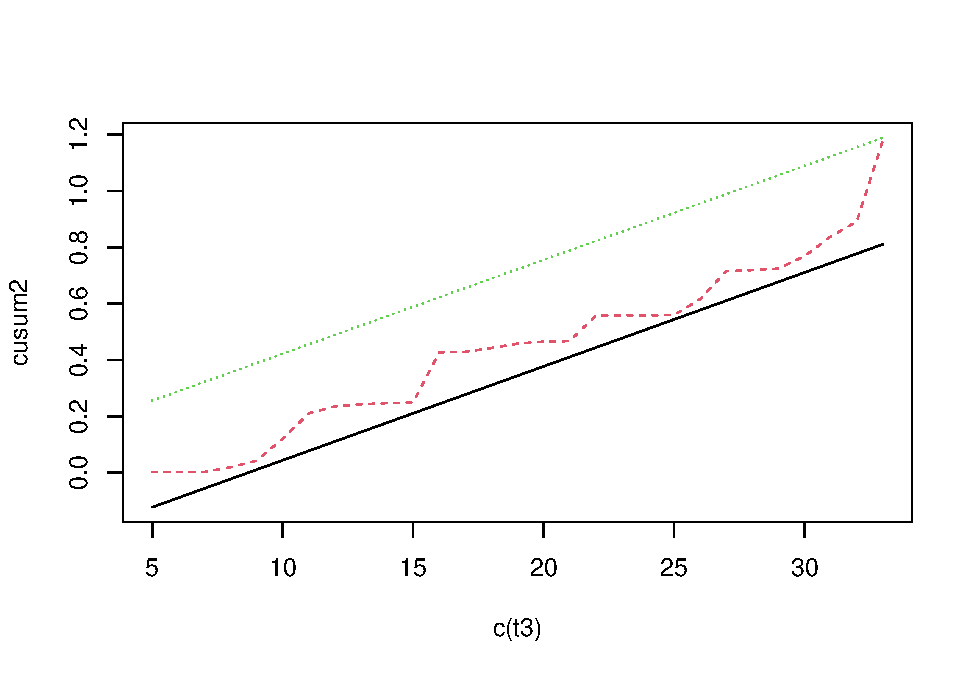
\includegraphics{Projet_econometrie_II_files/figure-latex/unnamed-chunk-14-1.pdf}

Fig. 12 : Test de Cusumsquare de stabilité temporelle du modèle 3

\hypertarget{test-dautocorruxe9lation-des-ruxe9sidus}{%
\subsubsection{Test d'autocorrélation des
résidus}\label{test-dautocorruxe9lation-des-ruxe9sidus}}

Le test de Breusch-Godrey permet de tester la significativité du
coefficient \(\rho\) qui représente l'autocorrélation des résidus :

\begin{equation}
    \label{eq:BG}
\varepsilon = \rho \varepsilon_{t-1} + u_t
\end{equation}

L'hypothèse nulle \(H_0\) revient à dire que \(\rho=0\), ie
l'autocorrélation est nulle. L'hypothèse laternative \(H_1\) suppose que
\(\rho \ne 0\), ie l'autocorrélation des résidus est existante. En
l'espèce, la p-value est signficaitive au seuil de 5\%, donc nous
rejettons l'hypothèse \(H_0\) d'absence d'autocorrélation.

\begin{longtable}[]{@{}
  >{\centering\arraybackslash}p{(\columnwidth - 4\tabcolsep) * \real{0.24}}
  >{\centering\arraybackslash}p{(\columnwidth - 4\tabcolsep) * \real{0.07}}
  >{\centering\arraybackslash}p{(\columnwidth - 4\tabcolsep) * \real{0.25}}@{}}
\caption{Breusch-Godfrey test for serial correlation of order up to 2:
\texttt{y\ \textasciitilde{}\ x}}\tabularnewline
\toprule
\begin{minipage}[b]{\linewidth}\centering
Test statistic
\end{minipage} & \begin{minipage}[b]{\linewidth}\centering
df
\end{minipage} & \begin{minipage}[b]{\linewidth}\centering
P value
\end{minipage} \\
\midrule
\endfirsthead
\toprule
\begin{minipage}[b]{\linewidth}\centering
Test statistic
\end{minipage} & \begin{minipage}[b]{\linewidth}\centering
df
\end{minipage} & \begin{minipage}[b]{\linewidth}\centering
P value
\end{minipage} \\
\midrule
\endhead
15.76 & 2 & 0.0003776 * * * \\
\bottomrule
\end{longtable}

\hypertarget{test-de-normalituxe9-des-ruxe9sidus}{%
\subsubsection{Test de normalité des
résidus}\label{test-de-normalituxe9-des-ruxe9sidus}}

La statistique de Jarque et Bera s'écrit :

\begin{equation}
    \label{eq:JB}
JB = \frac{T-(p+q)}{6} \left ( S^2 + \frac{1}{4}(K-3)^2 \right )
\end{equation}

L'hypothèse \(H_0\) de normalité des résidus revient à dire que :
\(JB \sim \chi^2\). La p-value n'est pas significative au seuil de 5\%.
Nous ne rejetons donc pas l'hypothèse nulle de normalité des résidus.

\begin{longtable}[]{@{}
  >{\centering\arraybackslash}p{(\columnwidth - 4\tabcolsep) * \real{0.24}}
  >{\centering\arraybackslash}p{(\columnwidth - 4\tabcolsep) * \real{0.07}}
  >{\centering\arraybackslash}p{(\columnwidth - 4\tabcolsep) * \real{0.14}}@{}}
\caption{Jarque Bera Test: \texttt{res}}\tabularnewline
\toprule
\begin{minipage}[b]{\linewidth}\centering
Test statistic
\end{minipage} & \begin{minipage}[b]{\linewidth}\centering
df
\end{minipage} & \begin{minipage}[b]{\linewidth}\centering
P value
\end{minipage} \\
\midrule
\endfirsthead
\toprule
\begin{minipage}[b]{\linewidth}\centering
Test statistic
\end{minipage} & \begin{minipage}[b]{\linewidth}\centering
df
\end{minipage} & \begin{minipage}[b]{\linewidth}\centering
P value
\end{minipage} \\
\midrule
\endhead
1.461 & 2 & 0.4816 \\
\bottomrule
\end{longtable}

\hypertarget{test-dhomoscuxe9dasticituxe9}{%
\subsubsection{Test
d'homoscédasticité}\label{test-dhomoscuxe9dasticituxe9}}

Nous utilisons le test de Breusch-Pagan pour analyser
l'hétéroscédasticité. En l'espèce, la p-value n'est pas significative au
seuil de 5\%. NOus ne rejetons pas l'hypothèse nulle d'homoscédasticité.

\begin{longtable}[]{@{}
  >{\centering\arraybackslash}p{(\columnwidth - 4\tabcolsep) * \real{0.24}}
  >{\centering\arraybackslash}p{(\columnwidth - 4\tabcolsep) * \real{0.07}}
  >{\centering\arraybackslash}p{(\columnwidth - 4\tabcolsep) * \real{0.14}}@{}}
\caption{studentized Breusch-Pagan test:
\texttt{y\ \textasciitilde{}\ x}}\tabularnewline
\toprule
\begin{minipage}[b]{\linewidth}\centering
Test statistic
\end{minipage} & \begin{minipage}[b]{\linewidth}\centering
df
\end{minipage} & \begin{minipage}[b]{\linewidth}\centering
P value
\end{minipage} \\
\midrule
\endfirsthead
\toprule
\begin{minipage}[b]{\linewidth}\centering
Test statistic
\end{minipage} & \begin{minipage}[b]{\linewidth}\centering
df
\end{minipage} & \begin{minipage}[b]{\linewidth}\centering
P value
\end{minipage} \\
\midrule
\endhead
7.619 & 4 & 0.1066 \\
\bottomrule
\end{longtable}

\hypertarget{pruxe9visions-uxe0-lhorizon-2025-uxe0-partir-du-moduxe8le-3}{%
\section{Prévisions à l'horizon 2025 à partir du modèle
3}\label{pruxe9visions-uxe0-lhorizon-2025-uxe0-partir-du-moduxe8le-3}}

Nous nous reposons sur le jeu d'hypothèse suivant sur les variables
explicatives. Celle-ci est basée sur un ensemble de scénarios concernant
les prix du diesel et du PIB.

\begin{table}[!h]

\caption{\label{tab:unnamed-chunk-18}valeur des variables explicatives de 2019 à 2025}
\centering
\fontsize{7}{9}\selectfont
\begin{tabu} to \linewidth {>{}r>{\raggedleft}X>{\raggedleft}X>{\raggedleft}X}
\toprule
Année & Prix du diesel déflaté 
\textbf{ du niveau général des prix} & \textbf{PIB en volume} & \textbf{Quantité de biens transportés par route}\\
\midrule
\textbf{2019} & 0.0130851 & 2331.980 & 322.3000\\
\textbf{2020} & 0.0122955 & 2366.593 & 318.4368\\
\textbf{2021} & 0.0109369 & 2503.562 & 310.7104\\
\textbf{2022} & 0.0103514 & 2602.636 & 317.5538\\
\textbf{2023} & 0.0112309 & 2653.216 & 339.6291\\
\textbf{2024} & 0.0129140 & 2690.018 & 350.2253\\
\textbf{2025} & 0.0127575 & 2723.548 & 355.7441\\
\bottomrule
\end{tabu}
\end{table}

La prédiction à partir des estimations du modèle 3 revient à calculer :

\[
\hat{y}_f = x_f' \tilde{\beta}
\]

A partir de la figure 13, nous remarquons que la consommation de gazole
par camion augmente. La consommation de gazole par camion en 2025 est de
22 888 milliers de tonnes.

\begin{table}[!h]

\caption{\label{tab:unnamed-chunk-19}Tableau des prévisions de 2019 à 2025}
\centering
\fontsize{7}{9}\selectfont
\begin{tabu} to \linewidth {>{}r>{\raggedleft}X>{\raggedleft}X>{\raggedleft}X>{\raggedleft}X}
\toprule
\textbf{Année} & \textbf{Valeur de la prévison} & \textbf{Borne inférieure} & \textbf{Borne supérieure} & \textbf{Ecart-type de prévision}\\
\midrule
\textbf{2019} & 19188.15 & 17991.34 & 20384.95 & 586.0169\\
\textbf{2020} & 19552.77 & 18313.19 & 20792.35 & 606.9632\\
\textbf{2021} & 20626.08 & 19105.00 & 22147.16 & 744.7982\\
\textbf{2022} & 21685.75 & 19974.69 & 23396.81 & 837.8221\\
\textbf{2023} & 22442.39 & 20817.47 & 24067.32 & 795.6448\\
\textbf{2024} & 22435.51 & 20906.54 & 23964.48 & 748.6606\\
\textbf{2025} & 22888.71 & 21318.02 & 24459.41 & 769.0916\\
\bottomrule
\end{tabu}
\end{table}

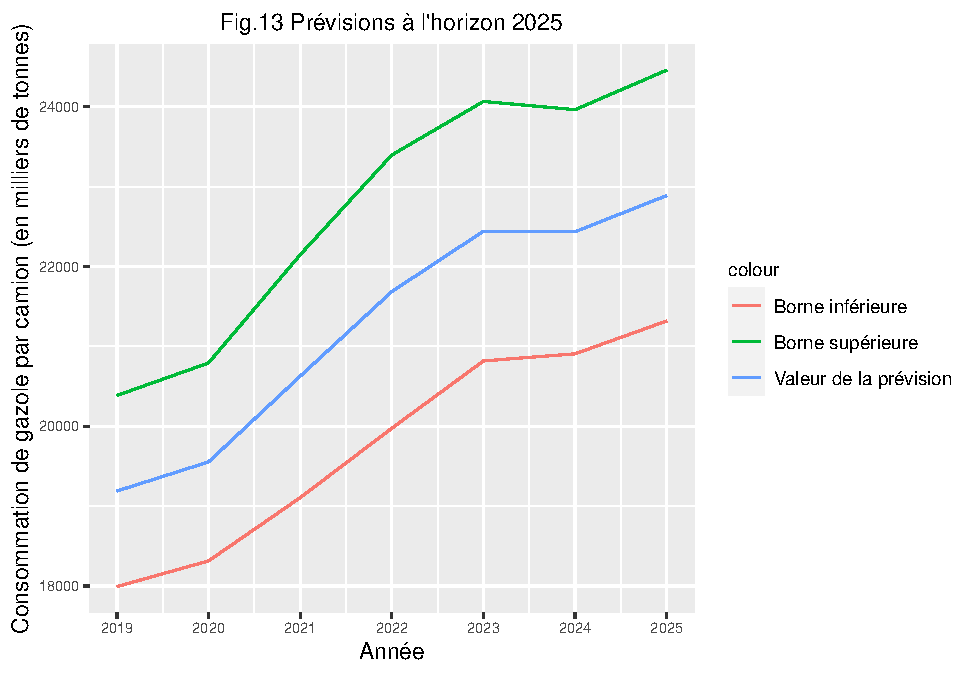
\includegraphics{Projet_econometrie_II_files/figure-latex/unnamed-chunk-20-1.pdf}

Nous calculons l'erreur quadratique moyenne, qui est de 2268 milliers de
tonnes par rapport à l'année 2019. Nous disposons, en effet, de la
valeur réelle de \(y\) en 2019.

\begin{verbatim}
## Valeur de l'erreur quadratique moyenne RMSE (sur les années 2018 et 2019) : 2268.731
\end{verbatim}

\printbibliography[title=Bibliographie]

\end{document}
